\chapter{The Approach of Horn and Schunck}
\chaptermark{The Approach of Horn and Schunck}
The research of Horn and Shunck has formed the basis of further research in the field of optical flow. They proposed the following quadratic penalized data term
\begin{align}
M(\textbf{w}) = (\nabla f^T \textbf{w} + f_t)^2,
\end{align}
which is equivalent to choosing
\begin{align*}
\Psi_M(\rho^2) = \rho^2
\end{align*}
in the framework of (\ref{DataPenalize}). The contribution to (\ref{EL}) from the model term is thus 
\begin{equation}
\begin{aligned}
\partial_{\textbf{w}} M = 2\nabla f(\nabla f ^T  \textbf{w} + f_t)
\end{aligned}
\end{equation}
The smoothness term used by Horn and Schunck is
\begin{align*}
V(\nabla u, \nabla v) = |\nabla u|^2 + |\nabla v|^2.
\end{align*}
This is a homogeneous regularizer which means that it applies an equal amount of diffusion in all directions. In the framework of (\ref{EL_regu}), this is equivalent to the diffusion matrices $\Theta_u$ and $\Theta_v$ being the identity matrix. Using this function as a flow regularizer gives
\begin{align*}
\partial_ {\textbf{w}_{x_i}} V = 2\textbf{w}_{x_i},
\end{align*}
for $x_i = x, y$. Dividing by 2 in all terms results in (\ref{EL}) taking the form 
\begin{equation}
\label{EL_HS}
\begin{aligned}
(f_x u + f_y v + f_t) f_x - \frac{1}{\sigma^2}(\frac{d}{d x} u_x + \frac{d}{d y} u_y ) &= 0  \quad \text{in} \ \Omega,  \\
(f_x u + f_y v + f_t) f_y - \frac{1}{\sigma^2}(\frac{d}{d x} v_x + \frac{d}{d y} v_y ) &= 0  \quad \text{in} \ \Omega  \\
\textbf{w}_{x} &= 0 \quad \text{on} \ \Gamma_e \ \text{and} \ \Gamma_w, \\
\textbf{w}_{y} &= 0 \quad \text{on} \ \Gamma_n \ \text{and} \ \Gamma_s,
\end{aligned}
\end{equation}
which can be seen as a system of coupled Poisson equations with Neumann boundary conditions:
\begin{align*}
-\frac{1}{\sigma^2} \Delta u + f_x ^2 u = - (F(v) + f_tf_x) \\
-\frac{1}{\sigma^2} \Delta v + f_y ^2 v = - (F(u) + f_tf_y) ,
\end{align*}
where $F(q) = f_xf_y q$.


\section{Discretizing the Horn and Schunck method}
\label{sec: disc}
Let now our image be of size m-by-n, and let $f^1$ and $f^2$ be the image at $t=1$ an $t=2$ respectively. Also, we flatten the regular 2-dimensional grid in $\Omega$ and consider now $(\xi^i)_ {i \in [mn]}$ so that $(\xi^i) = (x,y) = (\left \lfloor{i/m}\right \rfloor, i - \left \lfloor{i/m}\right \rfloor)$, when assuming the distance between vertical and horizontal grid points in $\Omega$ are 1. The corresponding vector representation of the image $f$ is denoted as $\textbf{f}(\xi^i) \in \mathbb{R}^{mn}$. Continuing this notation, the discrete flow values $\textbf{w}(\xi^i)$ is represented as the following vector in $\mathbb{R}^{2mn}$:
\begin{align*}
     \textbf{w}(\xi^i)=\begin{bmatrix}
         u(\xi^i)_{i\in [mn]}  \\
         v(\xi^i)_{i \in [mn]} \\
        \end{bmatrix}.
\end{align*}
For the discretization of the image gradients in (\ref{EL_HS}), the forward difference was used on $f^1$, producing the two vectors $\textbf{d}_x(\xi^i)$ and $\textbf{d}_y(\xi^i)$ in $\mathbb{R}^{mn)}$, where the gradients on the boundary are assumed to be zero. The time derivative $f_t$ is discretized using forward difference with time step $\Delta t = t_2 - t_1 = 1$ as shown below:
\begin{align*}
\textbf{c}(\xi^i) = \textbf{f}^2(\xi^i) - \textbf{f}^1(\xi^i),
\end{align*} 
where $\textbf{c}(\xi^i)$ is a vector in $\mathbb{R}^{mn}$. Normally when choosing derivative approximations one wants as high order as possible so that the truncation error goes to zero as one increases the number of grid points. In this case the number of grid points is fixed, so there is little to gain from choosing higher order approximations; it is best to choose the derivative approximation that results in the simplest discretization. Thus for the flow vector in (\ref{EL_HS}), the first derivative was approximated using backward difference, and the second was approximated using forward difference. Let now $L_x$ and $L_y$ be the matrices performing a forward difference on the components of the vector $\textbf{w}$ in $x$- and $y$-direction respectively. The gradient is then represented as
\begin{align*}
L \textbf{w}(\xi^i) = \begin{bmatrix}
         \tilde{u}_x(\xi^i)_{i\in [mn]}  \\
         \tilde{u}_y(\xi^i)_{i\in [mn]}  \\
         \tilde{v}_x(\xi^i)_{i\in [mn]} \\
         \tilde{v}_y (\xi^i)_{i\in [mn]} \\
        \end{bmatrix}
\end{align*}
where $\tilde{u}_x, \tilde{v}_x, \tilde{u}_y, \tilde{v}_y \in \mathbb{R}^{mn}$ are vector approximations to the derivatives. This means that $L$ is the following  block matrix:
\begin{align*}
L = \left[
\begin{array}{c c}
L_x & 0 \\
L_y & 0\\
0 & L_x \\
0 & L_y \\
\end{array}
\right].
\end{align*}

%\begin{align*}
%     \textbf{w}_x(\xi^i)=\begin{bmatrix}
%         u_x (\xi^i) \\
%         v_x (\xi^i)\\
%        \end{bmatrix} &\approx L_x \textbf{w}(\xi^i) = \begin{bmatrix}
%         \tilde{u}_x(\xi^i)  \\
%         \tilde{v}_x (\xi^i)\\
%        \end{bmatrix}  \\
%             \textbf{w}_y(\xi^i)=\begin{bmatrix}
%         u_y (\xi^i) \\
%         v_y (\xi^i)\\
%        \end{bmatrix} &\approx L_y \textbf{w}(\xi^i) = \begin{bmatrix}
%         \tilde{u}_y (\xi^i) \\
%         \tilde{v}_y(\xi^i) \\
%        \end{bmatrix},
%\end{align*} 
Since (\ref{EL_HS}) gives one set of equations for the interior nodes and one for the boundary nodes, these have to separated into two coupled systems. The interior system can be written as
\begin{align}
(D^T D + \frac{1}{\sigma^2} L^TL) \textbf{w}(\xi^i) = - D^T \textbf{c}(\xi^i),
\end{align}
for $(\xi^i) \in \Omega$ where $D$ is the block matrix
\begin{align*}
D = \left[
\begin{array}{c|c}
D_x & D_y
\end{array}
\right].
\end{align*}
$D_x$ and $D_y$ are diagonal matrices with the elements of $\textbf{d}_x(\xi^i)$ and $\textbf{d}_y(\xi^i)$ for $(\xi^i) \in \Omega$ along its diagonals respectively. When using a forward difference approximation of the derivative, the derivative approximations in the points next to $\Gamma_E$ and $\Gamma_S$ on the grid will be dependent on points on these boundaries respectively, and the derivative on these boundaries are set to zero. Let $\alpha(\xi^i) = (\textbf{d}_x(\xi^i) u(\xi^i) + \textbf{d}_y(\xi^i) v(\xi^i) + \textbf{c}(\xi^i))$. For $(\xi^{i+m}) \in \Gamma_E$ one gets 
\begin{align*}
\alpha(\xi^i) \textbf{d}_x(\xi^i) - \frac{1}{\sigma^2}\left[ L_x^T \left(u(\xi^i)-u(\xi^{(i+m)}) \right) + L_y^T \left( u(\xi^i)-u(\xi^{(i+1)}) \right) \right] &= 0 \\
\alpha(\xi^i) \textbf{d}_y(\xi^i) - \frac{1}{\sigma^2} \left[ L_x^T \left( v(\xi^i)-v(\xi^{(i+m)}) \right) + L_y^T \left( v(\xi^i)-v(\xi^{(i+1)}) \right) \right] &= 0,
\end{align*}
but since the derivative on the boundary is zero, one must enforce that $-L_x^Tq(\xi^{i+m}) = 0$ for $q = u,v$. This leads to
\begin{align*}
u(\xi^i) &= u(\xi^{(i+m)})  \\
v(\xi^i) &= v(\xi^{(i+m)}) 
\end{align*}
 so
\begin{align*}
\alpha(\xi^i) \textbf{d}_x(\xi^i) - \frac{1}{\sigma^2} L_y^T L_y u(\xi^i) &= 0 \\
\alpha(\xi^i) \textbf{d}_y(\xi^i) - \frac{1}{\sigma^2} L_y^T L_y v(\xi^i)  &= 0.
\end{align*}
Equivalently when $(\xi^{i+1}) \in \Gamma_S$,
\begin{align*}
u(\xi^i) &= u(\xi^{(i+1)})  \\
v(\xi^i) &= v(\xi^{(i+1)}) 
\end{align*}
which results in the following equations:
\begin{align*}
\alpha(\xi^i) \textbf{d}_x(\xi^i) - \frac{1}{\sigma^2} L_x^T L_x u(\xi^i) &= 0 \\
\alpha(\xi^i) \textbf{d}_y(\xi^i) - \frac{1}{\sigma^2} L_x^T L_x v(\xi^i) &= 0.
\end{align*}
On the two other boundaries $\Gamma_W$ and $\Gamma_N$, enforcing the forward differences to be zero at $(\xi^i) \in \Gamma_W$ leads to
\begin{align*}
u(\xi^i) &= u(\xi^{(i+m)})  \\
v(\xi^i) &= v(\xi^{(i+m)}), 
\end{align*}
and likewise for $(\xi^i) \in \Gamma_N$,
\begin{align*}
u(\xi^i) &= u(\xi^{(i+1)})  \\
v(\xi^i) &= v(\xi^{(i+1)}),.
\end{align*}


%The submatrix $L_x \in \mathbb{R}^{(m-2)(n-2) \times (m-2)(n-2)}$ is the block diagonal matrix
%\begin{align*}
%L_x = \left[
%\begin{array}{c|c|c|c|c}
%\epsilon_{m} & -\epsilon_{m} & 0 & \cdots& 0 \\ \hline
%0 &  I_{m} & -I_{m} & 0 & 0\\ \hline
%0 & 0 & \ddots & \ddots& 0 \\ \hline
%0 & \cdots & \cdots & 0_{m} & 0 _{m}
%\end{array}
%\right],
%\end{align*}
%where the last $n$ rows are zero owing to the....(bc) $L_y \in \mathbb{R}^{mn \times mn}$ the following band matrix:
%\begin{align*}
%L_y = \left[
%\begin{array}{c c c c}
%1 & -1 &  & \bigzero \\ 
% \bigzero & \ddots & \ddots &  \\
% &  & 1 & -1 \\
%\end{array}
%\right].
%\end{align*}
%The matrix multiplication with $L$ gives a forward difference approximation, and $-L^T$ gives a backward difference approximation. The matrix product $-L^TL$ is then the discretization of the second derivative in (\ref{EL_HS}).

\section{Results for the Horn and Schunck method}
The results when running the Horn and Schunck algorithm on our test images shown in Figures \ref{taxi1} and \ref{taxi2} for different regularization parameters are shown in Figure \ref{reguHS}. The choice of regularization parameter depends on the application, but one often want to get rid of most of the internal structure in each object, since these points will be moving with the same velocity (when assuming no deformation of the object). One also want to have a good enough balance between segmentation and smoothing. It is seen that choosing $\sigma = 0.003$ gives a fairly good segmentation of the objects that are moving, and with almost no internal structure. The flow field with this choice of regularization parameter is shown in Figure \ref{reguHS_best} on its own. The Horn and Schunck smoothes the flow in all directions, and the flow boundaries are therefore a bit smudged. 


\begin{figure}
\centering
\begin{minipage}{0.45\textwidth}
\centering
\includegraphics[scale=6]{{"/home/shomec/e/espenjv/Semester Project/Figures/taxi-00"}.eps}
\caption{First image in the Hamburg taxi sequence.}
\label{taxi1}
\end{minipage}\hfill
\begin{minipage}{0.45\textwidth}
\centering
\includegraphics[scale=6]{{"/home/shomec/e/espenjv/Semester Project/Figures/taxi-01"}.eps}
\caption{Second image in the Hamburg taxi sequence.}
\label{taxi2}
\end{minipage}
\end{figure}

%\begin{figure}
%    \centering
%    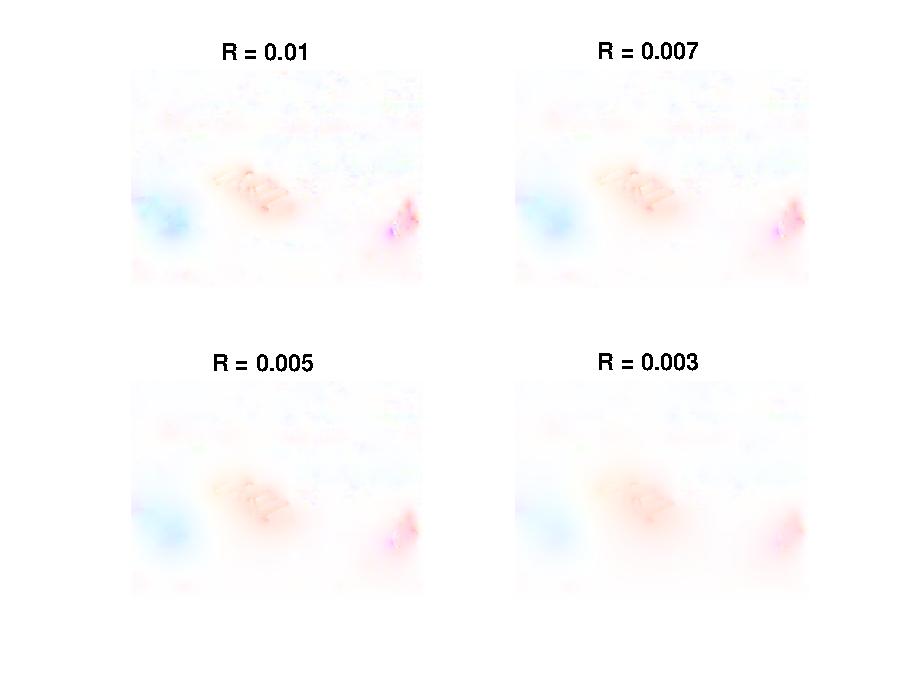
\includegraphics[scale=0.8]{regularizationHS}
%    \caption{Different choices for regularization parameter $\sigma$ using the Horn and Schunck algorithm}
%    \label{reguHS}
%\end{figure}
%
%\begin{figure}
%    \centering
%    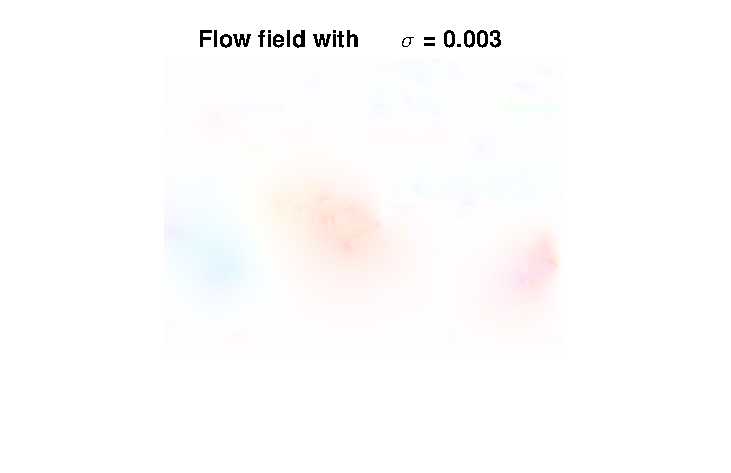
\includegraphics[scale=1]{HSregu}
%    \caption{Flow field with $\sigma= 0.003$ using the Horn and Schunck algorithm}
%    \label{reguHS_best}
%\end{figure}

